\documentclass{standalone}
\usepackage{graphicx}	
\usepackage{amssymb, amsmath}
\usepackage{color}

\usepackage{tikz}
\usetikzlibrary{intersections, backgrounds, patterns, patterns.meta}
\usepackage{pgfmath}

\definecolor{light}{RGB}{220, 188, 188}
\definecolor{mid}{RGB}{185, 124, 124}
\definecolor{dark}{RGB}{143, 39, 39}
\definecolor{highlight}{RGB}{180, 31, 180}
\definecolor{gray10}{gray}{0.1}
\definecolor{gray20}{gray}{0.2}
\definecolor{gray30}{gray}{0.3}
\definecolor{gray40}{gray}{0.4}
\definecolor{gray60}{gray}{0.6}
\definecolor{gray70}{gray}{0.7}
\definecolor{gray80}{gray}{0.8}
\definecolor{gray90}{gray}{0.9}
\definecolor{gray95}{gray}{0.95}

\begin{document}

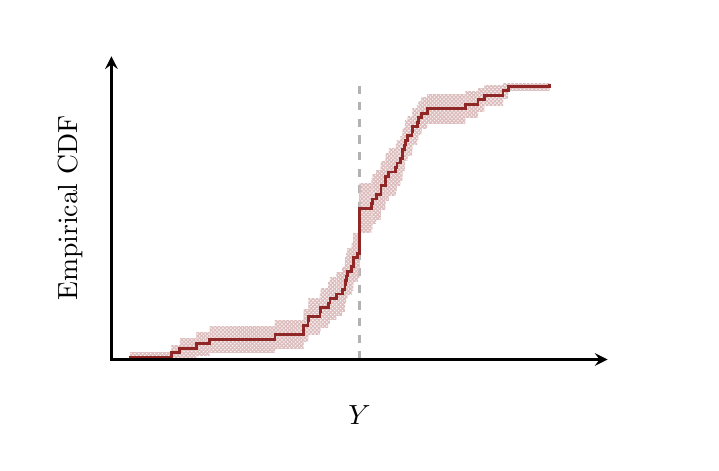
\begin{tikzpicture}[scale=0.35, thick]

\begin{scope}[shift={(0, 0)}]
  \draw[white] (-12, -3) rectangle (12, 12);

  \draw[dashed, gray70] (0, 0) -- (0, 10);

  \def\pgfmathsetglobalmacro#1#2{% 
    \pgfmathparse{#2}% 
    \global\let#1\pgfmathresult} 

  \pgfmathsetmacro{\previous}{-2.77513659846383} 
  
  \foreach \y [count=\n] in {-2.27513659846383, -2.27513659846383, -2.1727256420529, 
                             -2.1727256420529, -1.97294096508473, -1.97294096508473, -1.8139211603401, 
                             -1.8139211603401, -1.02219789733884, -1.02219789733884, -0.676432602801619,
                             -0.676432602801619, -0.67434906806149, -0.67434906806149, -0.621810995844637, 
                             -0.621810995844637, -0.618015204495698, -0.618015204495698, -0.477956759692787, 
                             -0.477956759692787, -0.470243936715443, -0.470243936715443, -0.378654844259842, 
                             -0.378654844259842, -0.357126097243555, -0.357126097243555, -0.278624376050029, 
                             -0.278624376050029, -0.209163059828732, -0.209163059828732, -0.175717686116424, 
                             -0.175717686116424, -0.172815863519913, -0.172815863519913, -0.161781335194661, 
                             -0.161781335194661, -0.145622681490234, -0.145622681490234, -0.0957773550648225, 
                             -0.0957773550648225, -0.0761096564142369, -0.0761096564142369, -0.0756303187976638, 
                             -0.0756303187976638, -0.0209052932950983, -0.0209052932950983, 0, 0, 0, 0, 0, 0,
                              0, 0, 0, 0, 0, 0, 0, 0, 0, 0, 0, 0, 0, 0, 0.143901398208538, 0.143901398208538, 
                              0.158721061223307, 0.158721061223307, 0.201094099262078, 0.201094099262078, 
                              0.258855469621821, 0.258855469621821, 0.259276964410342, 0.259276964410342, 
                              0.313446879008646, 0.313446879008646, 0.315500519454436, 0.315500519454436, 
                              0.35523772097357, 0.35523772097357, 0.438556062075263, 0.438556062075263, 
                              0.4535154991667, 0.4535154991667, 0.494943984606751, 0.494943984606751, 
                              0.519912141292594, 0.519912141292594, 0.521637253436326, 0.521637253436326, 
                              0.548764704923579, 0.548764704923579, 0.553229100326841, 0.553229100326841, 
                              0.581145990118473, 0.581145990118473, 0.63506678317272, 0.63506678317272, 
                              0.640874912449792, 0.640874912449792, 0.698384198028061, 0.698384198028061, 
                              0.712793742061684, 0.712793742061684, 0.749306520153625, 0.749306520153625, 
                              0.817888720686944, 0.817888720686944, 1.28196051102454, 1.28196051102454, 
                              1.43438564380133, 1.43438564380133, 1.50956396920404, 1.50956396920404, 
                              1.73665363540332, 1.73665363540332, 1.79856449975661, 1.79856449975661, 2.29856449975661} {
    
    \pgfmathsetmacro{\p}{(\n / 122.0}
    \pgfmathsetmacro{\delta}{sqrt(\p * (1 - \p) / 122.0)}
    \fill[pattern={Hatch[angle=45,distance=1, line width=0.5]}, pattern color=light] 
      (3 * \previous, {10 * max(0, \p - 2 * \delta)}) rectangle (3 * \y, {10 * min(1, \p + 2 * \delta)}); 
    \pgfmathsetglobalmacro{\previous}{\y}                           
  }
  
  \draw[dark, line width=1] (-9, 0) 
    \foreach \y [count=\n] in {-2.77513659846383, -2.27513659846383, -2.27513659846383, -2.1727256420529, 
                               -2.1727256420529, -1.97294096508473, -1.97294096508473, -1.8139211603401, 
                               -1.8139211603401, -1.02219789733884, -1.02219789733884, -0.676432602801619,
                               -0.676432602801619, -0.67434906806149, -0.67434906806149, -0.621810995844637, 
                               -0.621810995844637, -0.618015204495698, -0.618015204495698, -0.477956759692787, 
                               -0.477956759692787, -0.470243936715443, -0.470243936715443, -0.378654844259842, 
                               -0.378654844259842, -0.357126097243555, -0.357126097243555, -0.278624376050029, 
                               -0.278624376050029, -0.209163059828732, -0.209163059828732, -0.175717686116424, 
                               -0.175717686116424, -0.172815863519913, -0.172815863519913, -0.161781335194661, 
                               -0.161781335194661, -0.145622681490234, -0.145622681490234, -0.0957773550648225, 
                               -0.0957773550648225, -0.0761096564142369, -0.0761096564142369, -0.0756303187976638, 
                               -0.0756303187976638, -0.0209052932950983, -0.0209052932950983, 0, 0, 0, 0, 0, 0,
                                0, 0, 0, 0, 0, 0, 0, 0, 0, 0, 0, 0, 0, 0, 0.143901398208538, 0.143901398208538, 
                                0.158721061223307, 0.158721061223307, 0.201094099262078, 0.201094099262078, 
                                0.258855469621821, 0.258855469621821, 0.259276964410342, 0.259276964410342, 
                                0.313446879008646, 0.313446879008646, 0.315500519454436, 0.315500519454436, 
                                0.35523772097357, 0.35523772097357, 0.438556062075263, 0.438556062075263, 
                                0.4535154991667, 0.4535154991667, 0.494943984606751, 0.494943984606751, 
                                0.519912141292594, 0.519912141292594, 0.521637253436326, 0.521637253436326, 
                                0.548764704923579, 0.548764704923579, 0.553229100326841, 0.553229100326841, 
                                0.581145990118473, 0.581145990118473, 0.63506678317272, 0.63506678317272, 
                                0.640874912449792, 0.640874912449792, 0.698384198028061, 0.698384198028061, 
                                0.712793742061684, 0.712793742061684, 0.749306520153625, 0.749306520153625, 
                                0.817888720686944, 0.817888720686944, 1.28196051102454, 1.28196051102454, 
                                1.43438564380133, 1.43438564380133, 1.50956396920404, 1.50956396920404, 
                                1.73665363540332, 1.73665363540332, 1.79856449975661, 1.79856449975661, 2.29856449975661} {
    -- (3 * \y, {10 * (\n - 1) / 122.0}) -- (3 * \y, {10 * \n / 122.0})                          
  };

  \draw [->, >=stealth, line width=1] (-9, 0) -- (-9, 11);
  \node[rotate=90] at (-10.5, 5.5) { Empirical CDF };

  \draw [->, >=stealth, line width=1] (-9.05, 0) -- (9, 0);
  \node at (0, -2) { $Y$ };
  
\end{scope}
  
\end{tikzpicture}

\end{document}  